You are given the following data situation:
\begin{knitrout}
\definecolor{shadecolor}{rgb}{0.969, 0.969, 0.969}\color{fgcolor}\begin{kframe}
\begin{alltt}
\hlkwd{library}\hlstd{(ggplot2)}

\hlkwd{set.seed}\hlstd{(}\hlnum{123}\hlstd{)}

\hlcom{# generate 50 numerical observations with skewed error distribution (gamma)}
\hlstd{n} \hlkwb{=} \hlnum{50}
\hlstd{x} \hlkwb{=} \hlkwd{runif}\hlstd{(n)}
\hlstd{y} \hlkwb{=} \hlnum{2} \hlopt{*} \hlstd{x} \hlopt{+} \hlkwd{rgamma}\hlstd{(n,} \hlkwc{shape} \hlstd{=} \hlnum{1}\hlstd{)}

\hlkwd{ggplot}\hlstd{(}\hlkwd{data.frame}\hlstd{(}\hlkwc{x} \hlstd{= x,} \hlkwc{y} \hlstd{= y),} \hlkwd{aes}\hlstd{(}\hlkwc{x}\hlstd{=x,} \hlkwc{y}\hlstd{=y))} \hlopt{+}
  \hlkwd{geom_point}\hlstd{()}
\end{alltt}
\end{kframe}
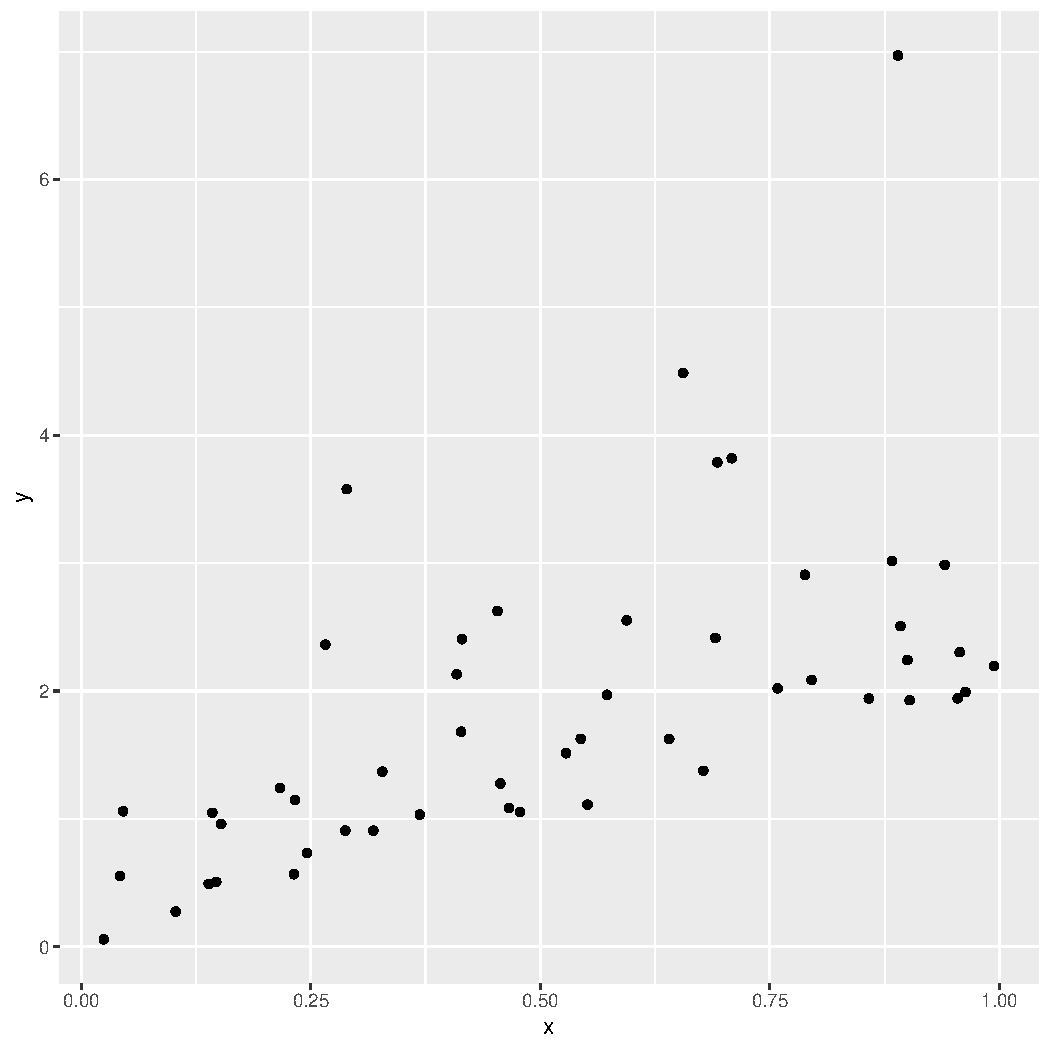
\includegraphics[width=0.5\linewidth]{figure/univ-plot-1} 
\end{knitrout}
\\ The general multivariate sparse quantile regression can be stated as in the lecture such as 
$$\min_{\beta\in\R^p}\underbrace{\frac{1}{n}\sum^n_{i = 1}\rho_\tau(y^{(i)} - \beta_0 -\bm{\beta}^\top\mathbf{x}^{(i)})}_{=\mathcal{R}_{\text{emp}}} \text{ s.t. } \Vert\bm{\beta}\Vert_1 \leq t$$
with $\tau \in (0, 1)$
$$\rho_\tau(s) = \begin{cases}\tau \cdot s & \text{for } s > 0 \\ 
-(1-\tau) \cdot s & \text{for } s \leq 0
\end{cases}$$
The $\rho_\tau(s)$ function is also called pinball loss. For $\tau \neq 0.5$, it asymmetrically assigns weights to the residuals:
\begin{knitrout}
\definecolor{shadecolor}{rgb}{0.969, 0.969, 0.969}\color{fgcolor}
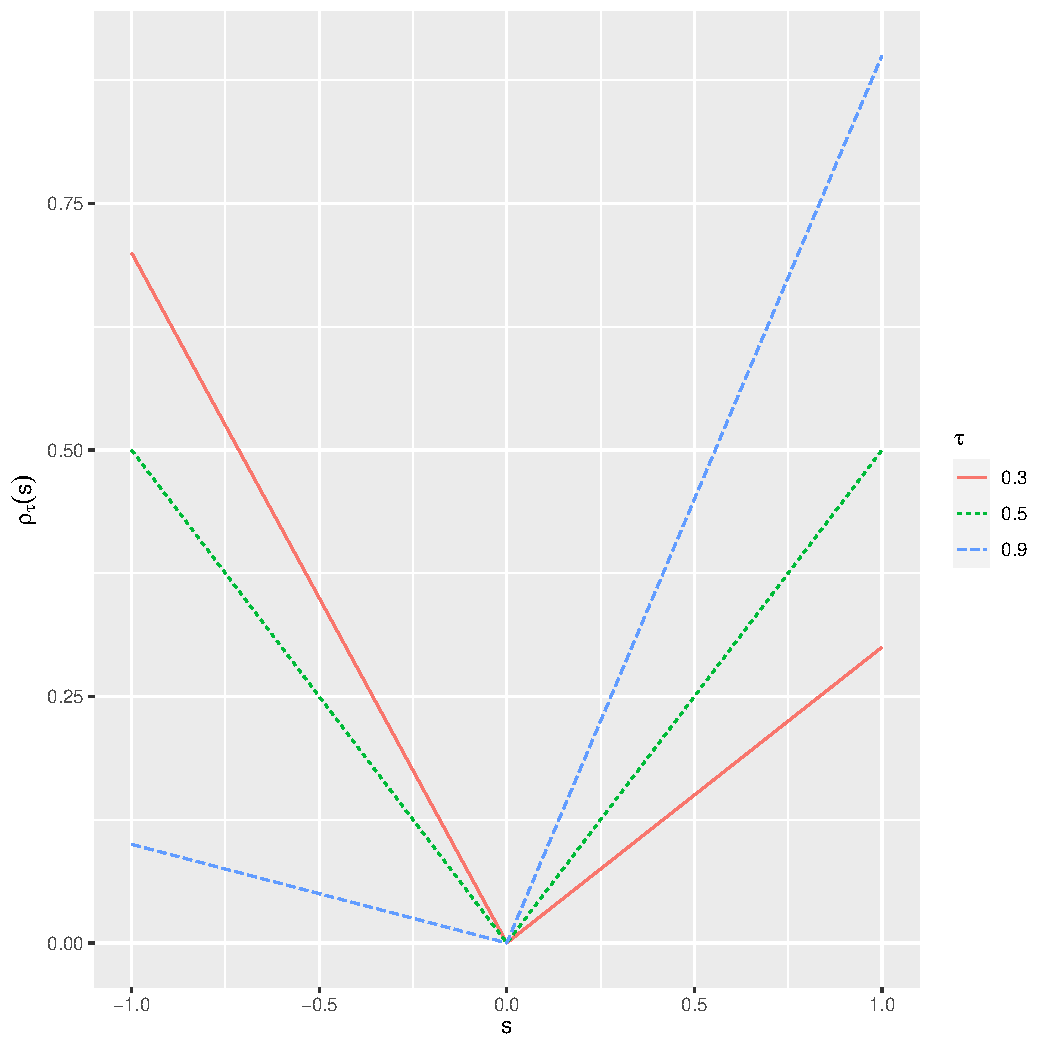
\includegraphics[width=0.5\linewidth]{figure/univ-pinball-1} 
\end{knitrout}

In the following we consider only the univariate case:
\begin{enumerate}
\item Find the standard form (as defined in the lecture) of the one-dimensional sparse quantile regression
\item Plot $\mathcal{R}_\text{emp}$ for $(\beta_0, \beta_1) \in [-3, 3]\times[-3, 3]$ and
$\tau = 0.4$ and mark the feasible region $(t = 1.7)$
\item Use the $\texttt{solveLP}$ command in $\texttt{R}$ to solve the sparse 40\% quantile regression $(t = 1.7)$
\item State the corresponding dual formulation of a) (as defined in the lecture)
\end{enumerate}
